\chapter{Boltzmann Machines}
The following chapter gives an introduction to Boltzmann machines and their applications to the classical 
simulation of quantum computing.

An overview of the architecture and mathematical properties of Boltzmann machines are given in the first section. The restricted Boltzmann machine is motivated as a special kind of Boltzmann machine with useful mathematical properties in the second part of this chapter. Afterward, the concepts of Gibbs sampling and supervised learning are explained.
In the last section, a constructive approach is given on how restricted Boltzmann machines 
can be applied to the classical simulation of quantum computing.

The introduction to Boltzmann machines and restricted Boltzmann machines as well as the introduction 
to Gibbs sampling are based on \cite{montufar2018restricted} and 
\cite{fischer2012introduction} which are also recommended as a more throughout introduction 
into the topic. The section on supervised learning and gradient descent methods is based on \cite{ruder2016overview}. The 
reader who is already familiar with the concept of Boltzmann machines and how they can be trained in a supervised 
manner can safely skip
to section~\ref{sec:applicationToQuantumComputing} which is based on the work of J\'{o}nsson, Bauer and Carleo \cite{jnsson2018neuralnetwork}.

\section{Overview}
The concept of the Boltzmann machine has first been proposed in the 1980s as a
model for parallel distributed computing \cite{hinton1983analyzing}. Boltzmann machines are physically inspired by the Ising Spin model and can be interpreted as energy-based recurrent neural networks representing probability distributions
over vectors $\bm{d}_i \in \{0,1\}^n$ \cite{ackley1985learning}.

A Boltzmann machine is a network of stochastic units (or neurons) $X=V \cup H$ which are segmented into
\textit{visible} neurons $V=\{v_1, \dots, v_n\}$ and \textit{hidden} neurons $H=\{h_1, \dots, h_m\}$.
The joint state of the visible neurons $\bm{v} = (v_1\dots v_n) \in \{0,1\}^n$ represents n-dimensional data
points $\bm{d}_i \in \{0,1\}^n$ while hidden neurons increase the expressiveness of the Boltzmann machine by acting as non-linear feature 
detectors to model dependencies between the visible neurons \cite{hinton2010boltzmann}.

The neurons are 
connected to each other by weighted links $W_{ij}$ and poss biases $a_i$ (visible) or $b_i$ (hidden) respectively. In the
general case, the neurons of a Boltzmann machine can be fully connected. A graphical representation of a fully connected Boltzmann machine is shown in figure~\ref{fig:boltzmannMachine}.

\begin{figure}[H]
    \label{fig:boltzmannMachine}
    \centering
    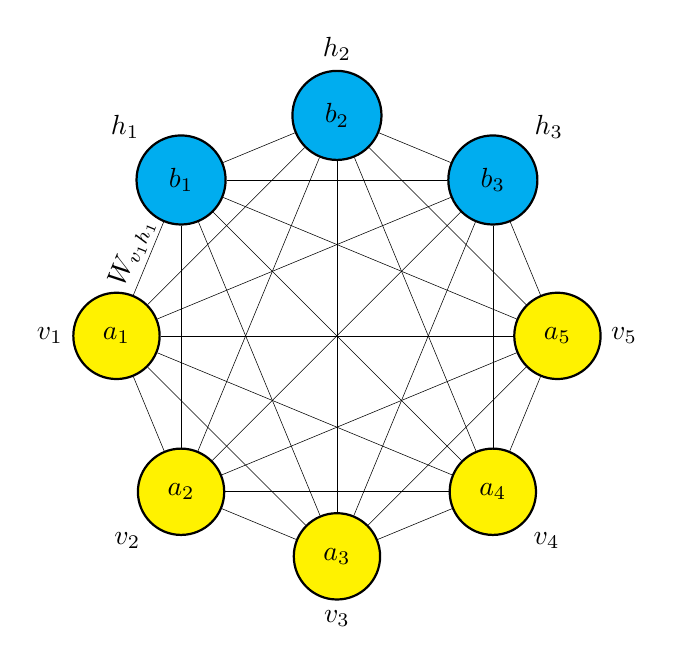
\begin{tikzpicture}[transform shape,line width=0.2pt]
        \foreach \x in {1,...,8}{%
            \pgfmathparse{(\x-1)*45+floor(\x/9)*22.5}
            \node[label={\pgfmathresult:\ifnum\x=1 $v_5$\else\ifnum\x=2 $h_3$\else\ifnum\x=3 $h_2$\else\ifnum\x=4 $h_1$\else\ifnum\x=5 $v_1$\else\ifnum\x=6 $v_2$\else\ifnum\x=7 $v_3$\else\ifnum\x=8 $v_4$\fi\fi\fi\fi\fi\fi\fi\fi},draw,circle,inner sep=0.25cm,fill={\ifnum\x=1 yellow\else\ifnum\x<5 cyan\else yellow\fi\fi}] (N-\x) at (\pgfmathresult:2.8cm) [thick] {\ifnum\x=1 $a_5$\else\ifnum\x=2 $b_3$\else\ifnum\x=3 $b_2$\else\ifnum\x=4 $b_1$\else\ifnum\x=5 $a_1$\else\ifnum\x=6 $a_2$\else\ifnum\x=7 $a_3$\else\ifnum\x=8 $a_4$\fi\fi\fi\fi\fi\fi\fi\fi};
        }
        \foreach \x [count=\xi from 1] in {2,...,8}{%
            \foreach \y in {\x,...,8}{%
                \ifnum\y=5 \else\ifnum\xi=5 \else \path (N-\xi) edge[-] (N-\y)\fi\fi;
            }
        }
        \draw (N-5) -- (N-1) node [] (E-1) {};
        \draw (N-5) -- (N-2) node [] (E-2) {};
        \draw (N-5) -- (N-3) node [] (E-3) {};
        \draw (N-5) -- (N-4) node [midway,above=-0.06cm,sloped] (E-4) {$W_{v_{1}h_{1}}$};
        \draw (N-5) -- (N-6) node [] (E-5) {}; 
        \draw (N-5) -- (N-7) node [] (E-6) {};
        \draw (N-5) -- (N-8) node [] (E-7) {};
    \end{tikzpicture}
    \caption{Graphical representation of a fully connected Boltzmann machine with 5 visible neurons (yellow) $v_1$ to $v_5$
    and 3 hidden neurons (blue) $h_1$ to $h_3$. Each neuron posses a bias
    $a_1$ to $a_5$ and $b_1$ to $b_3$ respectively. The connection weight between two neurons $i$ and $j$
    is given by $W_{ij}$.}
\end{figure}

Each configuration $\bm{c}=(v_1,\dots,v_n,h_1,\dots,h_m)$ of neuron states
of the Boltzmann machine is associated with an energy $E(\bm{c})$ value
which is defined by the parameters $\mathcal{W}$, consisting of its weights and 
biases $\mathcal{W} = \{a_i, b_i, W_{ij}\}$:

\begin{equation}
  E(\bm{c};\mathcal{W}) = - \sum_{v_i \in V} a_{i}v_{i} - \sum_{h_i \in H} b_{i}h_{i} - \sum_{x_i,x_j \in X} W_{x_i,x_j}x_{i}x_{j}
\end{equation}

When sampling configurations from the Boltzmann machine (discussed in more detail in section~\ref{sec:gibbsSampling}) the 
Boltzmann machines prefers low energy states over states with a high energy. The stationary probability
of a configuration $\bm{c}$ with energy $E(\bm{c};\mathcal{W})$ is given by the so called Gibbs-Boltzmann distribution \cite{gibbs_2010}:

\begin{equation}
   p(\bm{c};\mathcal{W}) = \frac{\mathrm{e}^{-E(\bm{c};\mathcal{W})}}{Z(\mathcal{W})}
\end{equation}

where $Z(\mathcal{W})$ is the normalizing partition function 

\begin{equation}
   Z(\mathcal{W}) = \sum_{\bm{c}\prime\in C} \mathrm{e}^{-E(\bm{c}\prime;\mathcal{W})}
\end{equation}

In a training phase (discussed in section~\ref{sec:learning} ) the parameters of the Boltzmann machine can be adapted in such a way that 
the marginal probability distribution of the visible neurons

\begin{equation}
    \label{eq:gbm}
   p(\bm{v};\mathcal{W}) = \sum_{\bm{h}_k \in \{0,1\}^m} p(\bm{v},\bm{h}_k;\mathcal{W})
\end{equation}

,which traces out the hidden unit 
states by summing over all possible configurations of them, resembles the probability 
distribution of data points $\bm{d}_i$ in a training set $D=\{d_1,\dots,d_l\}$.

For a fully connected Boltzmann machine, this representation consists of an exponential number of summands and cannot be calculated efficiently. So-called Restricted Boltzmann machines
(RBM) have a specific architecture with a restricted connectivity, which allows calculating the marginal probability to be efficient. RBMs and their architectures will be explained in the next section.

\section{Restricted Boltzmann machines}
The so-called Restricted Boltzmann machine (RBM) is an important type of Boltzmann machine with 
a specific architecture and properties \cite{smolensky1986information}. Since their invention, RBMs have been applied to a variety 
of machine learning tasks and played a 
key role in the development of deep learning architectures as building blocks of so-called 
Deep Belief networks \cite{bengio2009learning, hinton2006fast}.
RBMs are also the kind of Boltzmann machines which are being used in this study for the simulation 
of quantum circuits.

In the restricted case, the neurons of the Boltzmann machine are separated into two layers,
one being the visible layer containing the visible neurons $v_i \in V$ and the other layer being the hidden layer containing the hidden neurons $h_j \in H$. Each neuron of the RBM 
is only allowed to be connected to the neurons from the other layer. Intra-layer connections are not allowed, making the graph of the RBM bipartite, as shown in figure~\ref{fig:rbm}. 

\begin{figure}[H]
    \label{fig:rbm}
    \centering
    \begin{tikzpicture}[transform shape,line width=0.2pt]
    
        \node (v1)[neuron, fill=yellow] at (0, 0) {$a_1$};
        \node (v2)[neuron, fill=yellow] at (2, 0) {$a_2$};
        \node (v3)[neuron, fill=yellow] at (4, 0) {$a_3$};
        \node (v4)[neuron, fill=yellow] at (6, 0) {$a_4$};
        \node[below=0.1cm of v1] (bv1) {$v_1$};
        \node[below=0.1cm of v2] (bv2) {$v_2$};
        \node[below=0.1cm of v3] (bv3) {$v_3$};
        \node[below=0.1cm of v4] (bv4) {$v_4$};
    
        \node (h1)[neuron, fill=cyan] at (1, 2) {$b_1$};
        \node (h2)[neuron, fill=cyan] at (3, 2) {$b_2$};
        \node (h3)[neuron, fill=cyan] at (5, 2) {$b_3$};
        \node[above=0.1cm of h1] (bh1) {$h_1$};
        \node[above=0.1cm of h2] (bh2) {$h_2$};
        \node[above=0.1cm of h3] (bh3) {$h_3$};
    
        \draw (v1) -- (h1) node [midway,above=-0.06cm,sloped] {$W_{v_1h_1}$};
        \draw (v1) -- (h2) node [midway,above=-0.06cm,sloped] {};
        \draw (v1) -- (h3) node [midway,above=-0.06cm,sloped] {};
    
        \draw (v2) -- (h1) node [midway,above=-0.06cm,sloped] {};
        \draw (v2) -- (h2) node [midway,above=-0.06cm,sloped] {};
        \draw (v2) -- (h3) node [midway,above=-0.06cm,sloped] {};
    
        \draw (v3) -- (h1) node [midway,above=-0.06cm,sloped] {};
        \draw (v3) -- (h2) node [midway,above=-0.06cm,sloped] {};
        \draw (v3) -- (h3) node [midway,above=-0.06cm,sloped] {};
    
        \draw (v4) -- (h1) node [midway,above=-0.06cm,sloped] {};
        \draw (v4) -- (h2) node [midway,above=-0.06cm,sloped] {};
        \draw (v4) -- (h3) node [midway,above=-0.06cm,sloped] {};
    \end{tikzpicture}
    \caption{Graphical representation of a RBM with 5 visible neurons and 3 hidden ones. 
    There are only connections between the two layers and no connection between two neurons 
    from the same layer.}
\end{figure}

The marginal probability of the visible neuron states in a RBM has the form:

\begin{align}
   p(\bm{v};\mathcal{W}) &= \sum_{\bm{h}_k \in \{0,1\}^m} p(\bm{v},\bm{h}_k;\mathcal{W})\\
   &= \frac{1}{Z(\mathcal{W})}\sum_{\bm{h}_k \in \{0,1\}^m} \mathrm{e}^{-E(\bm{v}, \bm{h}_k;\mathcal{W})}\\
   &= \frac{1}{Z(\mathcal{W})}\sum_{h_1\in \{0,1\}}\dots\sum_{h_m \in \{0,1\}}\mathrm{e}^{\sum_{v_i}b_iv_i}\prod_{j=1}^m\mathrm{e}^{h_j(b_j + \sum_{i=1}^nW_{ij}v_i)}\\
   &= \frac{\mathrm{e}^{\sum_{v_i}b_iv_i}}{Z(\mathcal{W})}\sum_{h_1 \in \{0,1\}}\mathrm{e}^{h_1(b_1 + \sum_{i=1}^nW_{i1}v_i)}\dots\sum_{h_m \in \{0,1\}}\mathrm{e}^{h_m(b_m + \sum_{i=1}^nW_{im}v_i)}\\
   &= \frac{\mathrm{e}^{\sum_{v_i}b_iv_i}}{Z(\mathcal{W})}\prod_{i=1}^m\sum_{h_i \in \{0,1\}}\mathrm{e}^{h_i(b_i + \sum_{i=1}^nW_{ij}v_i)}\\
   \label{eq:rbm}
   &= \frac{\mathrm{e}^{\sum_{v_i}b_iv_i}}{Z(\mathcal{W})}\prod_{i=1}^m(1+\mathrm{e}^{b_i + \sum_{i=1}^nW_{ij}v_i}).
\end{align}

This quantity consists of only a polynomial number of terms in the number of hidden units of the RBM and can be calculated efficiently. This makes the RBM a compact representation of a probability distribution over vectors $\bm{d}_i \in D$ inferred from a dataset $D$.

Even though the RBM has a limited connectivity between its units, it is a universal function approximator \cite{le2008representational}.
It can model any distribution over $\{0,1\}^m$ arbitrary well with $m$ visible and $k+1$ hidden units, where 
$k$ denotes the cardinality of the support set of the target distribution, that is, the number of input elements
from $\{0,1\}^m$ that have a non-zero probability of being observed. This also implies a worst-case 
exponential number of hidden units for distributions with an extensive support set \cite{le2008representational}. It has been shown though that even fewer units can be sufficient depending on the patterns in the support set \cite{montufar2011refinements}.

\section{Gibbs Sampling}
\label{sec:gibbsSampling}

Boltzmann machines are generative models representing probability distributions over their configurations. This means that it is possible to draw configurations from a Boltzmann machine
according to their (marginal) probabilities given in equations~\ref{eq:gbm} and \ref{eq:rbm}.

Though it is required to calculate $Z(\mathcal{W})$ for the exact probabilities of each configuration,
it is not necessary to calculate the energies for all the $2^{n+m}$ possible configurations of 
a Boltzmann machine to draw samples from it.

Instead, Boltzmann machines can be seen as \textit{Markov chains} with a \textit{stationary probability
distribution}. With a stochastic process called \textit{Gibbs sampling} the samples can be drawn efficiently according to this stationary distribution for RBMs.

This section gives a short introduction into Markov chains, Gibbs sampling and how it can be applied 
to draw configurations from an RBM.

Gibbs sampling belongs to the class of so-called \textit{Metropolis-Hastings} algorithms and by that is 
a \textit{Monte Carlo Markov Chain} (MCMC) algorithm \cite{hastings1970monte}. It is a simple algorithm to produce samples from the joint probability distribution of multiple random variables like neuron state configurations
of a Boltzmann machine, which can be considered as a Markov chain.

A Markov chain is a discrete stochastic process of configurations of random variables $C=\{\bm{c}^{(t)}\}$
at time steps $t=1, \dots, T$ which take values in a set $\Omega$ (for Boltzmann machines 
$\Omega=\{0,1\}^{m+n}$) and for which for all time steps $t$ and for all configurations 
$\bm{c}_j, \bm{c}_i, \bm{c}_{i-1}, \dots, \bm{c}_0 \in \Omega$ the \textit{Markov property} holds:

\begin{align}
    p_{ij}^{(t)} &:= P(\bm{c}^{(t+1)} = c_j \mid \bm{c}^{(t)} = \bm{c}_i, \dots, \bm{c}^{(0)} = c_0) \\
                 & = P(\bm{c}^{(t+1)} = c_j \mid \bm{c}^{(t)} = \bm{c}_i) 
\end{align}

meaning that the next state of the system only depends on the current state and not on the system's history. A Markov chain can be represented as a (finite) graph as the one shown in figure~\ref{fig:markov}.

\begin{figure}[H]
    \label{fig:markov}
    \centering
    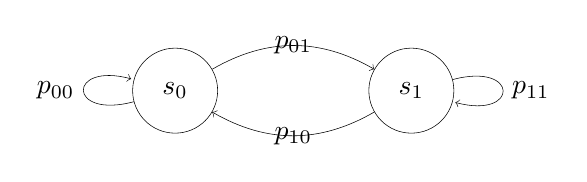
\begin{tikzpicture}[transform shape,line width=0.2pt]
    
        \node [draw,circle,inner sep=0.25cm] (s0) at (0,0) {$s_0$};
        \node [draw,circle,inner sep=0.25cm] (s1) at (3,0) {$s_1$};
    
        \path[->] (s0) edge[loop left]  node {$p_{00}$} (s0);
        \path[->] (s0) edge[bend left] node {$p_{01}$} (s1);
        \path[->] (s1) edge[bend left] node {$p_{10}$} (s0);
        \path[->] (s1) edge[loop right] node {$p_{11}$} (s1);
    
    \end{tikzpicture}
    \caption{A Markov chain with two possible states $c_0$ and $c_1$. The Markov chain is 
described by the $2 \times 2$ matrix $\bm{P}=\dots$}
\end{figure}

In the case of Boltzmann machines the transition probabilities $p_{ij}$ are time independent and 
given by the ratios of configuration probabilities. For RBMs the transition probability $p_{ij}$ 
from configuration $c_i$ to $c_j$ is given by:

\begin{equation}
    p_{ij} = \frac{\mathrm{e}^{\sum_{v_i \in \bm{c_i}}b_iv_i}\prod_{i=1}^m(1+\mathrm{e}^{b_i + \sum_{i=1}^nW_{ij}v_i})}{\mathrm{e}^{\sum_{v_i \in \bm{c_j}}b_iv_i}\prod_{i=1}^m(1+\mathrm{e}^{b_i + \sum_{i=1}^nW_{ij}v_i})}
\end{equation}

which can be calculated efficiently as the $Z(\mathcal{W})$ terms from equation~\ref{eq:rbm} cancel out.

In each time step $t$ during the Gibbs sampling, the state of a single randomly chosen neuron of the RBM is flipped
so that the configurations $\bm{c}^{(t)}$ and $bm{c}^{(t+1)}$ only differ in the state of one neuron. With 
probability $p_{ij}$ configuration $\bm{c}_j$ is kept as the new configuration and with probability
$1-p_{ij}$ the Boltzmann machine will stay in its current configuration $bm{c}_i$. This corresponds to a random walk on the Markov chain defined by the RBM transition probabilities. The algorithm is given in 
algorithm~\ref{alg:gibbs}.

\begin{algorithm}[H]
    \label{alg:gibbs}
    \caption{Gibbs Sampling}\label{euclid}
    \begin{algorithmic}[1]
        \Require $bm(c)$: function returning the energy of a Boltzmann machine for configuration $c$
        \Require T: time steps
        \State $t\gets 0$
        \State $c^{(0)} \gets randomize(\{0,1\}^{m+n})$ (random initialization)
        \Repeat
            \State $r \gets random(m+n)$
            \State $E_i \gets bm(c^{(t)})$
            \State $E_j \gets bm(\{c_1,\dots,\bar{c_r},\dots,c_{m+n}\})$
            \If{$random(1) < \frac{E_i}{E_j}$}
                \State $c^{(t+1)} \gets \{c_1,\dots,\bar{c_r},\dots,c_{m+n}\}$
            \EndIf
            \State $t\gets t+1$
        \Until{$t=T$}
        \State \textbf{return} $c^{(T)}$
    \end{algorithmic}
\end{algorithm}

The Markov chain for configurations of a Boltzmann machine is known to converge to its so-called 
\textit{stationary distribution} $\pi$, that is

\begin{equation}
    \pi^T=\pi^T\bm{P}
\end{equation}

with $\bm{P} = (p_{ij})$ being the transition matrix of the Markov chain with the transition probabilities as its entries.
Once the Markov chain reaches its stationary distribution, all subsequent states will be distributed according to this distribution.

This means running Gibbs sampling for 
sufficiently many time steps $T$ will sample configurations according 
to the Gibbs-Boltzmann distribution given in equation~\ref{eq:rbm}.

Although Gibbs sampling is a straightforward algorithm, it is an important algorithm in the context of 
Boltzmann machines. Different versions of Gibbs sampling have been developed for RBMs like 
(persistent) contrastive divergence \cite{hinton2002training, tieleman2008training} or parallel tempering \cite{desjardins2010parallel}. In this study,
Gibbs sampling will be used in its simplest version, as described in this chapter.
    
\section{Supervised Learning}
\label{sec:learning}
The probability distribution over vector spaces given by a Boltzmann machine can be trained to 
resemble the distribution of data points $\bm{d}_i$ in a dataset $D=\{\bm{d}_1,\dots,\bm{d}_d\}$. This can be done either in a \textit{unsupervised}
or in a \textit{supervised} manner.

In both cases the parameters $\mathcal{W} = \{\bm{a},\bm{b},\bm{W}\}$ of the Boltzmann machine are updated minimizing 
an objective function $O(\mathcal{W})$ which depends on the parameters of the Boltzmann machine and 
depicts the overlap of the current and the target distribution in an iterative process called 
\textit{gradient descent}.

This section gives a brief introduction into supervised learning and the gradient descent method \textit{Adamax} \cite{kingma2014adam}.

Before the training phase, the Boltzmann machine is initialized with random parameters and a training set 
$D=\{\bm{d}_1,\dots,\bm{d}_d\}$ is given. In the case of supervised learning of Boltzmann machines, the training set consists of tuples of configurations and their corresponding target energy values $\bm{d}_i= (\bm{c}_i, t_i)$.

In the batch version of gradient descent, which is being used in this study, the training set $D$ is 
split into subsets $D_1, \dots, D_l$, also called \textit{batches}.

For each such batch $D_i$, the average overlap $O(\bm{c}_j; \mathcal{W})$ for all $\bm{c}_j \in D_i$
is computed. Afterwards, the gradients $\Delta O_{x}$ are calculated and the parameters updated into
the direction of the steepest descent:

\begin{equation}
    \label{eq:sgd}
    \Theta_i = \Theta_i + \Delta O \dots.
\end{equation}

This process is repeated for a defined number of iterations to minimize the objective function $O(\mathcal{W})$.
A graphical representation of this process is shown in figure~\ref{fig:sgd}.

\begin{figure}[H]
    \label{fig:sgd}
    \centering
    \begin{tikzpicture}[transform shape,line width=0.2pt]
    
        \draw[->] (0,0) -- (3,0) node[right] {$x$};
        \draw[->] (0,0) -- (0,2) node[above] {$y$};
        \draw[scale=0.01,domain=0:10,smooth,variable=\x,blue] plot ({\x},{(\x-10)^2+10});
    
    \end{tikzpicture}
    \caption{Iterations of gradient descent.} 
\end{figure}

The simple update rule in \ref{eq:sgd} has several drawbacks, however. First, The gradient and thus the step size will become smaller as closer the function approaches its minimum, leading to only small improvements and many steps necessary.
Second, the function's shape will usually have (many) local minima, which should be avoided.
Several variants of gradient descent have been developed to overcome these issues \cite{ruder2016overview}.

One successful such strategy which is used in this study is called \textit{AdaMax}, a special version 
of \textit{Adam} \cite{kingma2014adam}.It combines the advantages of AdaGrad \cite{duchi2011adaptive} and RMSProp \cite{bengio2015rmsprop},
two other popular gradient descent methods. It is computationally efficient, has little
memory requirements, and proves to be well suited for problems with much noise and sparse gradients.

The algorithm updates exponential moving averages of the gradient ($mt$) and the squared gradient
($vt$) where the hyper-parameters $\beta_1, \beta_2 \in [0, 1)$ control the exponential decay rates of these moving
averages. The moving averages themselves are estimates of the 1st moment (the mean) and the
2nd raw moment (the uncentered variance) of the gradient. The update rule for the parameters $\Theta_{ij}$ for Adamax are summarized in 
algorithm~\ref{alg:adamax}.

\begin{algorithm}
    \label{alg:adamax}
    \caption{Adamax}\label{euclid}
    \begin{algorithmic}[1]
        \Require $\alpha$: step size
        \Require $\beta_1, \beta_2 \in [0,1)$: Exponential decay rates
        \Require $f(\Theta)$: Stochastic objective function with parameters $Theta$
        \Require $\Theta_0$: Initial parameter vector
        \State $m_0 \gets 0$ (Initialize $1^{st}$ moment vector)
        \State $u_0 \gets 0$ (Initialize the exponential weighted infinity norm)
        \State $t \gets 0$ (Initialize time step)
        \While {$\Theta_t$ not converged}
            \State $t\gets t+1$
            \State $g_t \gets \nabla_{\Theta}f_t(\Theta_{t-1})$ (Get gradients w.r.t. objective function at time step $t$)
            \State $m_t \gets \beta_1 \cdot m_{t-1} + (1-\beta_1) \cdot g_t$ (Update biased first moment estimate)
            \State $u_t \gets max(\beta_2 \cdot u_{t-1}, \vert{g_t})$ (Update the exponentially weighted infinity norm)
            \State $\Theta_t \gets \Theta_{t-1} - (\alpha/ (1-\beta_1^t)) \cdot m_t/u_t$ (Update parameters)
        \EndWhile
        \State \textbf{return} $\Theta_t$ (Resulting parameters)
    \end{algorithmic}
\end{algorithm}

\section{Application to Quantum Computing}
\label{sec:applicationToQuantumComputing}
Machine learning techniques have become a successful approach for the classical simulation
of quantum systems \cite{carleo2017solving, deng2017quantum, carleo2018constructing}. 
Carleo and Troyer \cite{carleo2017solving} have first given a compact presentation of the wavefunction of a many-body quantum system with an RBM.
The same framework has later been used by J\'{o}nsson, Bauer, and Carleo for the classical simulation of the quantum Fourier and Hadamard transform \cite{jnsson2018neuralnetwork}. Their work gives a constructive approach on how the parameters of a complex-valued RBM representing the quantum state

\begin{equation}
   \Psi_{\mathcal{W}}(\mathcal{B}) = \frac{\mathrm{e}^{\sum_{v_i}b_iv_i}}{Z(\mathcal{W})}\prod_{i=1}^m(1+\mathrm{e}^{b_i + \sum_{i=1}^nW_{ij}v_i})
\end{equation}

can be adapted to apply a universal set of quantum gates to the quantum state $\Psi_{\mathcal{W}}$.

RBMs allow only an exact application of unitary gates diagonal in the computational basis. For non-diagonal 
gates more hidden layers would be necessary, making the calculation of the quantum state intractable \cite{carleo2018constructing}. Nevertheless, it is possible to train a Boltzmann machine in a supervised fashion, so its parameters are adapted to apply a non-diagonal gate to its state approximately.

The rules for the applications of diagonal and non-diagonal gates to an RBM state from 
\cite{jnsson2018neuralnetwork} detailed in following two sections.

\subsection{Diagonal gates}

Diagonal gates can be applied to an RBM quantum state by solving a set of linear equations. 
This section describes the rules for the applications of single-qubit Z rotations, controlled Z rotations 
as well as the Pauli X, Y and Z gates.

\subsubsection{Single-Qubit Z rotations}
The action of the single Z rotation of angle $\theta$ is given by the $2\times2$ unitary matrix

\begin{equation}
    \begin{pmatrix}
        1 & 0 \\
        0 & \mathrm{e}^{i\theta}
    \end{pmatrix} .
\end{equation}

Its action on qubit $l$ yields 
$\langle \mathcal{B} \mid R_{l}^{z}(\theta) \mid \Psi_{W}  \rangle = 
\mathrm{e}^{i\theta B_{l}} \Psi_{W}(\mathcal{B})
$
. Considering a RBM machine with weights $\mathcal{W}\prime = \{\alpha,\beta,W\}$, the action of the $R^{Z}{\theta}$
gate is exactly reproduced if $\mathrm{e}^{B_{l}a_{l}}\mathrm{e}^{i\theta B_{l}} = \mathrm{e}^{B_{l}a\prime_{l}}$
is satisfied, which is the case for:

\begin{equation}
    a\prime_{j} = a_{j} + \delta_{jl}i\theta
\end{equation}

The action of the Z rotation thus simply modifies the bias of the visible neuron $l$ of the RBM.

\subsubsection{Controlled Z rotations}
The action of a controlled Z rotations acting on two given qubits $l$ and $m$ is determined by
the $4\times4$ unitary matrix:

\begin{equation}
    \begin{pmatrix}
        1 & 0 & 0 & 0 \\
        0 & 1 & 0 & 0 \\
        0 & 0 & 1 & 0 \\
        0 & 0 & 0 & \mathrm{e}^{i\theta}
    \end{pmatrix}
\end{equation}

where $\theta$ is a given rotation angle. This gate is diagonal and can compactly be written as an 
effective two-body interaction:

\begin{equation}
    \langle \mathcal{B} \mid CZ(\theta) \mid \Psi_{W}  \rangle = 
    \mathrm{e}^{i\theta B_{l}B_{m}}\Psi_{W}(Z_{1} \dots Z_{N}).
\end{equation}

As the RBM architecture does not allow direct interaction between visible neurons, the CZ gate
requires the insertion of a dedicated extra hidden unit $h_{c}$ which is connected
to the qubits $l$ and $m$: 

\begin{align}
    \langle \mathcal{B} \mid CZ(\theta) \mid \Psi_{W}  \rangle &= 
    \mathrm{e}^{\Delta a_{l} B_{l} + \Delta a_{m} Z_{m}} \sum_{h_{c}}\mathrm{e}^{W_{lc} B_{l} h_{c} + W_{mc} B_{m} h_{c}} \\
    &= \mathrm{e}^{\Delta a_{l} B_{l} + \Delta a_{m} B_{m}} \times (1 + \mathrm{e}^{W_{lc} B_{l} + W_{mc}} B_{m}) \Psi_{W}(\mathcal{B}),
\end{align}

where the new weights $W_{lc}$ and $W_{mc}$ and visible units biases $a_{l}\prime= a_{l} + \Delta a_{l}$,
$a_{m}\prime= a_{m} + \Delta a_{m}$ are determined by the equation:

\begin{equation}
   \mathrm{e}^{\Delta a_{l} B_{l} + \Delta a_{m} B_{m}}(1 + \mathrm{e}^{W_{lc} B_{l} + W_{mc} B_{m}}) = C \times \mathrm{e}^{i \theta B_{l} B_{m}}
\end{equation}

for all the four possible values of the qubits values $B_{l}, B_{m} = \{0,1\}$ and where $C$ is an arbitrary (finite)
normalization. A possible solution for this system is:

\begin{equation}
   W_{lc} = -2\mathrm{A}(\theta) 
\end{equation}

\begin{equation}
   W_{mc} = 2\mathrm{A}(\theta) 
\end{equation}

\begin{equation}
   \Delta a_{l} = i \frac{\theta}{2} + \mathrm{A}(\theta)
\end{equation}

\begin{equation}
   \Delta a_{m} = i \frac{\theta}{2} - \mathrm{A}(\theta)
\end{equation}

where $\mathrm{A}(\theta) = arccosh(\mathrm{e}^{-i \frac{\theta}{2}})$

\subsubsection{Pauli X gate}
The X gate just flips the qubit $l$ and the RBM amplitudes are:

$
    \langle \mathcal{B} \mid X_{l} \mid \Psi_{W}  \rangle = 
    \langle B_{1} \dots \bar{B_{l}} \dots B_{N} \mid \Psi_{W} \rangle.
$

Since $\bar{B_{l}} = (1-B_{l})$, it must be satisfied that

\begin{equation}
    (1-B_{l})W_{lk} + b_{k} = B_{l} W_{lk}\prime + b_{k}\prime
\end{equation}

and

\begin{equation}
   (1-B_{l}) a_{l} = B_{l} a_{l}\prime + C 
\end{equation}

hold for all the (two) possible values of $B_{l} = \{0,1\}$. The solution is simply:

\begin{equation}
   W_{lk}\prime = -W_{lk}
\end{equation}

\begin{equation}
   b_{k}\prime = b_{k} + W_{lk}
\end{equation}

\begin{equation}
   a_{l}\prime = -a_{l}
\end{equation}

\begin{equation}
   C = a_{l}
\end{equation}

whereas all the $a_{j}$ and the other weights $W_{jk}$ with $j \neq i$ are unchanged.

\subsubsection{Pauli Y gate}
A similar solution is also found for the $Y$ gate, with the noticeable addition of extra phases
with respect to the $X$ gate:

\begin{equation}
   W_{lk}\prime = -W_{lk}
\end{equation}

\begin{equation}
   b_{k}\prime = b_{k} + W_{lk}
\end{equation}

\begin{equation}
   a_{l}\prime = -a_{l} + i \pi
\end{equation}

\begin{equation}
   C = a_{l} + \frac{i \pi}{2}
\end{equation}

whereas all the $a_{j}$ and other weights $W_{jk}$ with $j \neq l$ are unchanged.

\subsubsection{Pauli Z gate}
The Pauli Z gate is a special case of the Z rotation with $\theta = \pi$. Thus the 
only change necessary is to set the bias $a_l$ of the visible neuron $l$ to

\begin{equation}
    a_{l}\prime = a_{l} + i \pi.
\end{equation}

\subsection{Non-diagonal gates}

Exact applications of non-diagonal gates to Boltzmann machine quantum states would require introducing a second hidden layer \cite{carleo2018constructing}. In contrast to an RBM with just one hidden layer, this would make the calculation of the represented quantum state inefficient.

Thus there are no rules for applying non-diagonal gates to an RBM state similar to those for diagonal gates. Nevertheless, the parameters of the RBM can be adapted in a 
supervised learning process instead.

The training set consists of samples drawn from the RBM with its current set of parameters. In the sampling process, the RBM's energy function can be adapted to resemble the energy states after a non-diagonal unitary gate $ G $ has been applied to its state.

For any non-diagonal unitary gate

\begin{equation}
    G =  \begin{pmatrix}
        a & b \\
        c & d
    \end{pmatrix}
\end{equation}

applied to qubit $l$ samples from the state $\ket{\Phi(\mathcal{B})} = G_l\ket{\Psi(\mathcal{B})}$ can be drawn according to 

\begin{equation}
    \lvert \ket{\Phi(\mathcal{B}_{\mathcal{B}_l = 0})} \rvert^2 = 
    \lvert  a \cdot \ket{\Psi(\mathcal{B}_{\mathcal{B}_l = 0})} +
            c \cdot \ket{\Psi(\mathcal{B}_{\mathcal{B}_l = 1})}
    \rvert^2
\end{equation}

when the state of qubit $l$ is sampled to be 0 and 

\begin{equation}
    \lvert \ket{\Phi(\mathcal{B}_{\mathcal{B}_l = 1})} \rvert^2 = 
    \lvert  b \cdot \ket{\Psi(\mathcal{B}_{\mathcal{B}_l = 0})} +
            d \cdot \ket{\Psi(\mathcal{B}_{\mathcal{B}_l = 1})}
    \rvert^2
\end{equation}

when the state is sampled to be 1. The sampling happens according to the squared norm
$\lvert \Phi \rvert^2$ to draw the samples according to the probability distribution of the 
corresponding quantum state.

The samples are then being used to minimize the log-likelihood of the overlap of the two quantum 
states $\Psi$ and $\Phi$

\begin{align}
    L(\mathcal{W}) &= -\log{O(\mathcal{W})} \\
                   &= -\log{\sqrt{\frac{\lvert \Braket{\Psi_{\mathcal{W}}|\Phi} \rvert^2}{\Braket{\Psi_{\mathcal{W}}|\Psi_{\mathcal{W}}} \Braket{\Phi|\Phi}}}}\\
                   &= -\log{\sqrt{\Bigg\langle \frac{\Phi(\mathcal{B})}{\Psi_{\mathcal{W}}(\mathcal{B})} \bigg \rangle_{\Psi} \Bigg\langle \frac{\Psi_{\mathcal{W}}(\mathcal{B})}{\Phi(\mathcal{B})} \bigg \rangle_{\Phi}^{*}}}
\end{align}

with

\begin{equation}
    \langle F(\mathcal{B})\rangle_A := \frac{\sum_{\mathcal{B}} F(\mathcal{B}) \lvert A(\mathcal{B}) \rvert^2}{\sum_{\mathcal{B}} \lvert A(\mathcal{B})\rvert^2}
\end{equation}

by a gradient descent method. The gradients of this function with respect to 
the parameters of the Boltzmann machine have the following form:

\begin{equation}
   \partial_{p_k}L(\mathcal{W}) = \langle \mathcal{O}_k^*(\mathcal{B}) \rangle_{\Psi} - \frac{\langle \frac{\Phi(\mathcal{B})}{\Psi(\mathcal{B})} \mathcal{O}_k^*(\mathcal{B})\rangle_{\Psi}}{\langle \frac{\Phi(\mathcal{B})}{\Psi(\mathcal{B})} \rangle_{\Psi}}
\end{equation}

with $\mathcal{O}_k(\mathcal{B}) = \partial_{p_k}\log{\Psi_{\mathcal{W}}(\mathcal{B})}$ being the variational derivatives of the RBMs wavefunction with respect to its parameters.
These are simple to compute as well:

\begin{equation}
    \partial_{a_i}\log{\Psi_{\mathcal{W}}(\mathcal{B})} = v_i
\end{equation}

\begin{equation}
    \partial_{b_i}\log{\Psi_{\mathcal{W}}(\mathcal{B})} = h_i
\end{equation}

\begin{equation}
    \partial_{W_{ij}}\log{\Psi_{\mathcal{W}}(\mathcal{B})} = v_ih_j
\end{equation}

After the training, which happens for a predefined number of iterations on batches of the training set,
the quantum state $\Psi_{\mathcal{W}}$ represented by the RBM approximates the target state $\Phi$. Using
this approach J\'{o}nsson et al. reported a per gate error of $10^{-3}$ \cite{jnsson2018neuralnetwork}.